
%(BEGIN_QUESTION)
% Copyright 2011, Tony R. Kuphaldt, released under the Creative Commons Attribution License (v 1.0)
% This means you may do almost anything with this work of mine, so long as you give me proper credit

PT-58, PRC-58, and PV-58 comprise a gas pressure control system to monitor and regulate gas pressure in this oil/natural-gas separator vessel by venting excess natural gas to the flare.  During normal operation, there is just a little bit of gas flow vented to the flare.  Most of the gas exits the separator vessel through control valve FV-66:

$$\includegraphics[width=15.5cm]{i03565x01.eps}$$

Suppose one day you are asked to remove PT-58 from service and take it back to the shop for a routine calibration check, while allowing operators to continue to run the separator.  Identify what you would have to physically do in this system to prepare the transmitter for safe removal (i.e. the steps you would have to take up to the point of removing the bolts attaching PT-58 to its manifold), including any interactions you should have with the operations personnel after being approved to enter into the process area.

\underbar{file i03565}
%(END_QUESTION)





%(BEGIN_ANSWER)

\noindent
3 points for having operator place controller in manual mode (monitoring pressure via PG-11), 2 points for having operator disable low-pressure alarm (or informing the operator that the pressure reading will fail low), and 5 points for correct valve manifold procedure:

\vskip 10pt

Close the high-side block valve and open the equalizing valve.  The low-side block valve may be left open or closed.

%(END_ANSWER)





%(BEGIN_NOTES)

{\bf This question is intended for exams only and not worksheets!}.

%(END_NOTES)


